% NB: use pdflatex to compile NOT pdftex.  Also make sure youngtab is
% there...

% converting eps graphics to pdf with ps2pdf generates way too much
% whitespace in the resulting pdf, so crop with pdfcrop
% cf. http://www.cora.nwra.com/~stockwel/rgspages/pdftips/pdftips.shtml




\documentclass[10pt,aspectratio=169]{beamer}
%\usetheme[everytitleformat=uppercase]{m}
\usetheme[everytitleformat=regular,color/block=transparent]{m}
\usepackage[absolute,overlay]{textpos}
\usepackage{booktabs}

\usepackage{graphbox} %loads graphicx package

\usepackage{pbox}

\usepackage{adjustbox}

\usepackage[utf8]{inputenc}


\usepackage[scale=2]{ccicons}


\usepackage[official]{eurosym}



%use this to add space between rows
\newcommand{\ra}[1]{\renewcommand{\arraystretch}{#1}}

% for sources http://tex.stackexchange.com/questions/48473/best-way-to-give-sources-of-images-used-in-a-beamer-presentation

\setbeamercolor{framesource}{fg=gray}
\setbeamerfont{framesource}{size=\tiny}


\newcommand{\source}[1]{\begin{textblock*}{4cm}(11.7cm,8.0cm)
    \begin{beamercolorbox}[ht=0.5cm,right]{framesource}
        \usebeamerfont{framesource}\usebeamercolor[fg]{framesource} Source: {#1}
    \end{beamercolorbox}
\end{textblock*}}

\usepackage{hyperref}


%\usepackage[pdftex]{graphicx}


\graphicspath{{graphics/}}

\DeclareGraphicsExtensions{.pdf,.jpeg,.png,.jpg}



\let\olditem\item
\renewcommand{\item}{%
\olditem\vspace{5pt}}

\title{
}
%\subtitle{---}
\author{
  \emph{Tom Brown, The Open Energy Modelling Community}
}

\date{\vspace{0.5cm}Open Power System Data Workshop, Berlin, 10th July 2017}


\titlegraphic{%
  \vspace{0.7cm}
  % left bottom right top
  
\includegraphics[width=12.5cm]{openmod-logo-vector}

}



\begin{document}

\maketitle

\begin{frame}
  \frametitle{openmod: overview}

\begin{itemize}
  \item \alert{grass roots community} of open energy modellers from universities
  and research institutions
  \item participants mainly from Europe, but also from Africa, America,
    and Australia
  \item first meeting Berlin 18–19 September 2014 as an off-shoot of
    strommarkttreffen (some founding members started OPSD)
  \item promoting \alert{open code}, \alert{open data} and \alert{open science}
\end{itemize}
\end{frame}


\begin{frame}
  \frametitle{what is open modelling?}

  \centering
  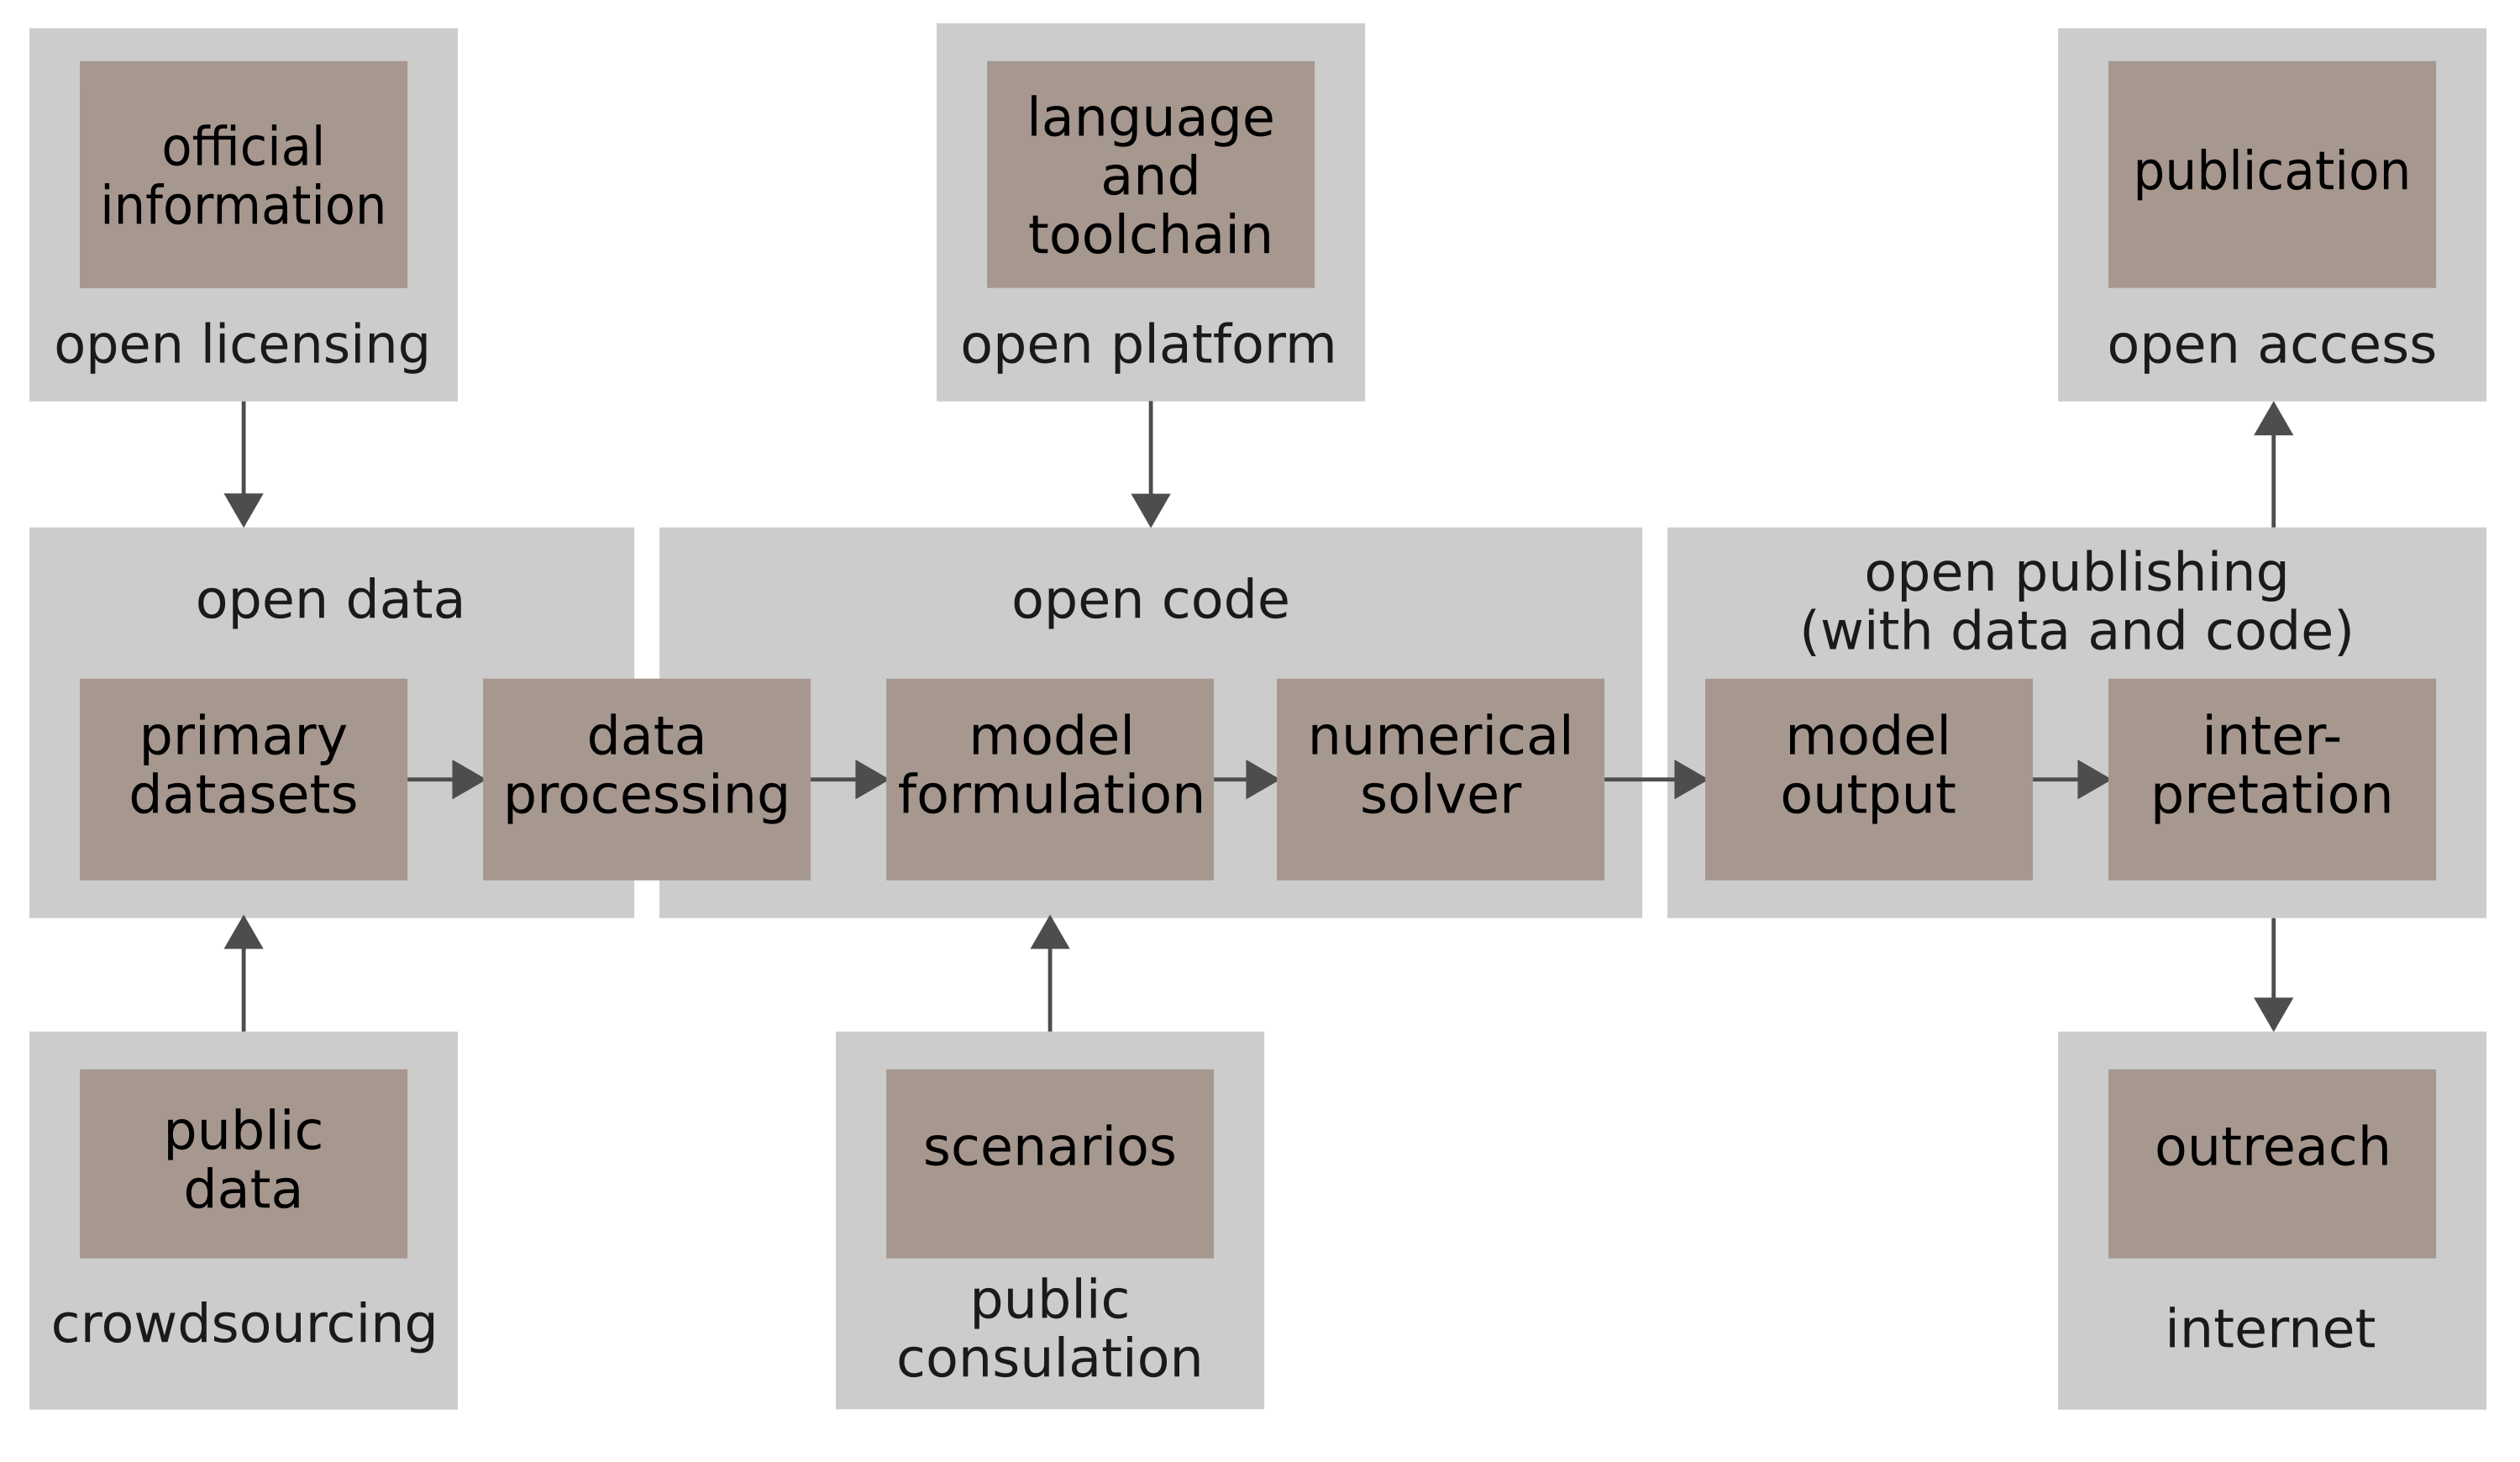
\includegraphics[width=12.5cm]{open-modeling-chain}

  \source{Robbie Morrison, Eva Schmid, CC 4.0 BY}
\end{frame}


\begin{frame}
  \frametitle{why open modelling?}

  openness \dots
  \begin{itemize}
  \item \dots increases \alert{transparency}, \alert{reproducibility} and
    \alert{credibility}, which lead to better research and policy
    advice
  \item \dots \emph{can} improve research \alert{quality}
  \item  \dots reduces
    \alert{duplication of effort} and frees time for the development of
    \alert{new ideas}
  \item \dots allows easier \alert{collaboration}
  \end{itemize}
  \end{frame}

\begin{frame}{Copyright}


  Unless otherwise stated, the graphics and text are Copyright \copyright Tom Brown, 2017.

  The graphics and text for which no other attribution are given are licensed under a
  \href{http://creativecommons.org/licenses/by/4.0/}{Creative Commons
  Attribution 4.0 International Licence}.

  \begin{center}\ccby\end{center}

\end{frame}

\end{document}
